%!TEX root = ../../Compte-rendu.tex

\begin{figure}[H]
	\begin{center}
		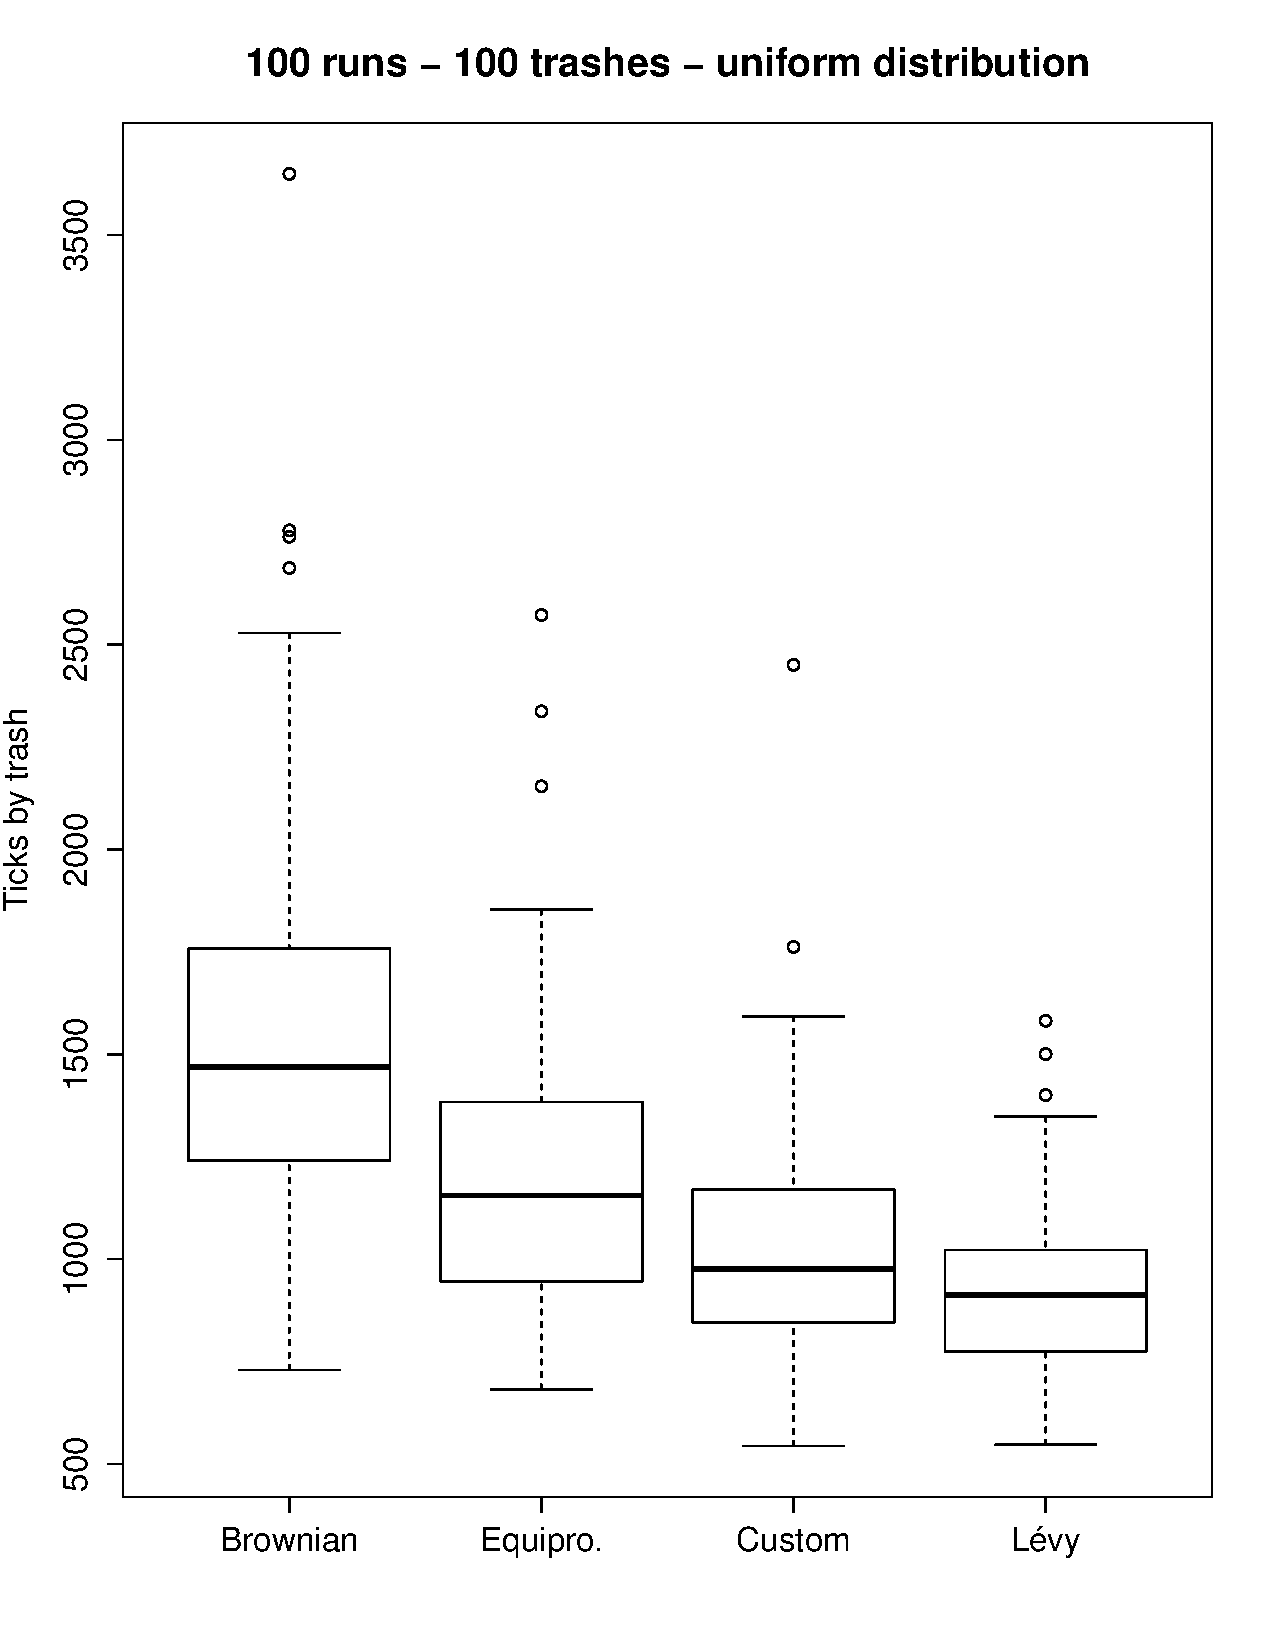
\includegraphics[height=10cm]{diagrams/100TrRnd_all.pdf}
		\caption{Résultat des mesures pour 100 débris uniformément répartis}
		\label{fig:100Trashes_Rnd}
	\end{center}
\end{figure}

Nous avons pour les différentes stratégies les médianes suivantes :

\begin{figure}[H]
	\begin{center}
		\begin{tabular}{ | c | c | }
			\hline
			Brownian & 1468.673 \\
			Equiprobable & 1155.213 \\
			Custom & 974.9208 \\
			Lévy & 911.797 \\
			\hline
		\end{tabular}
		\caption{Médianes pour 100 débris distribués uniformément}
	\end{center}
\end{figure}
